\documentclass[10pt]{article}


%\usepackage[letterpaper, 
%			top    = 20mm, 
%			bottom = 25mm,
%			left   = 30mm,
%			right  = 30mm]{geometry}
			
%\usepackage[parfill]{parskip}		% Avoids the skip at start of new paragraph
\usepackage{graphicx}
\usepackage{amssymb}
\usepackage{amsmath}
\usepackage[usenames,dvipsnames]{xcolor} % https://en.wikibooks.org/wiki/LaTeX/Colors
%\usepackage{xspace}
%\usepackage{natbib}

%\usepackage{float} % Place figures exactly "here" (option "H")

%\usepackage[useregional]{datetime2}	% \DTMnow
\usepackage{lastpage} 				% \pageref{LastPage}

\usepackage[]{hyperref}
%\hypersetup{
%    colorlinks,
%    linkcolor={black},
%    citecolor={blue!80!black},
%    urlcolor={Aquamarine}
%}

%\usepackage[font={small,it}]{caption} 
%\captionsetup[table]{skip=10pt}

\usepackage{lineno}
%\linenumbers

% Bibliography:
% apalike: display author names
% plain: just a number, ordered by appeareance
\bibliographystyle{apalike}


%\usepackage{authblk}
%\renewcommand\Affilfont{\itshape\small}

% ===== HEADERS / FOOTERS =====
%\usepackage{fancyhdr}
%\setlength{\headheight}{15.2pt}
%\fancyhead[L]{Modelling Sequence Uncertainty}
%\fancyhead[C]{}
%\fancyhead[R]{Champredon, Becker, Chato, Gugan, and Poon}
%\renewcommand{\headrulewidth}{0.8pt}
%\fancyfoot[L]{\footnotesize\DTMnow}
%\fancyfoot[C]{\thepage \, / \pageref{LastPage}}
%%\fancyfoot[R]{ \textcolor{red}{DRAFT}}
%\renewcommand{\footrulewidth}{0.4pt}
%\pagestyle{fancy}
% ==============================




% ==== GENERAL ====

\newcommand{\warning}[1]{\textbf{\textcolor{orange}{((#1))}}}
\newcommand{\comment}[1]{\textsl{\textcolor{cyan}{((#1))}}}
\newcommand{\eg}{\textit{e.g.,}\xspace}
\newcommand{\ie}{\textit{i.e.},\xspace}

% ==== SPECIFIC ====

\newcommand{\sq}[1]{\texttt{\textcolor{brown}{#1}}}

\newcommand{\sps}{\mathcal{B}} % sequence probability sequence
\newcommand{\nps}{\mathcal{S}} % nucleotide probability sequence
\newcommand{\nlps}{nucleotide-level probabilistic sequence\xspace}
\newcommand{\slps}{sequence-level probabilistic sequence\xspace}

\newcommand{\pr}[1]{\mathbb{P}(#1)}

\newcommand{\md}{\mathcal{M}} % Multinomial distribution
\newcommand{\pois}[1]{\mathrm{Poisson}\left(#1\right)}
\newcommand{\betadist}[1]{\mathrm{Beta}\left(#1\right)}




% ===================

\begin{document}

\Huge
\textsf{Modelling Sequence Uncertainty}

\large
\vspace{1cm}

David Champredon and Art Poon\\
\small
Western University, London, Ontario, Canada.

\vspace{1cm}
\normalsize
\begin{center}
\today
\end{center}


\linenumbers
%\modulolinenumbers[2]


\normalsize
\vspace{1cm}
\tableofcontents

\newpage

\section{Introduction}


\textbf{Sequencing error.} 
Extracting DNA/RNA from biological samples is a complex process that involves several steps: extraction of the genetic material of interest (avoiding contamination with foreign/unwanted genetic material); reverse transcription (if RNA); DNA fragmentation of the genome into smaller segments; amplification of the fragmented sequences using PCR; sequencing the fragments (\eg with fluorescent techniques); putting back the small fragments together by aligning them (de novo) or mapping them to benchmark libraries.\comment{(all this must be checked by someone who knows well the process!)}
Errors can be introduced at each of these steps for various reasons \cite{Beerenwinkel:2011} and some errors can be quantified (\eg sequencing quality scores from chromatographs). 

\textbf{In-host diversity and polymorphisms.} 
When the phylogenic tree to infer is based on pathogen sequences infecting hosts, the potential genetic diversity of the infection adds a complexity in phylogeny reconstruction. Typical examples are epidemiological studies reconstructing transmission trees from viral genetic sequences (\eg HIV, HepC) sampled from infected patients \comment{ref phyloscanner}. 


\textbf{Current uncertainty management.} 
The different sources of uncertainty described above impact our observations of the actual genetic sequences.
There are standard approaches to deal with identifiable observation errors. 
Base calls that are ambiguous (from equivocal chromatograph curves or because of genuine polymorphisms) are assigned ambiguity codes (\eg Y for C or T, R for A or G, etc.).
Alignment methods are heuristic methods based on similarity scores that generally do not quantify the uncertainty of alignment.\comment{double check this is indeed the case for MUSCLE, MAPFT, PRANK, ClustalW}
Methods to reconstruct phylogenies usually leave out the uncertainty complexity and settle for sequences composed of the most frequent nucleotides and/or ignore ambiguity codes.

\textbf{Propagate and quantify uncertainty.}
In summary, sources of sequencing observation errors are known and, for a few of them, quantified (quality scores, ambiguity codes).
But, to our knowledge, the resulting uncertainty has never been propagated and quantified in a statistical framework for downstream analysis (\eg alignments,  phylogenies inferences).
\comment{Check what BALIphy does, this may be the only example of uncertainty propagation}
In other words, genetic sequences are treated as \emph{certain} quantities.

\vspace*{1ex}

Here we propose a theoretical framework to represent genetic sequence uncertainty and quantify the impact of uncertainty as it is propagated through methods of phylogeny reconstruction. 



% ==============================================================
% ==============================================================


\newpage

\section{Methods}


In the first part of this section, we propose two simple probabilistic frameworks to represent the uncertainty of genetic sequences observations.
The second part describes how those theoretical frameworks can be practically informed from data.


\subsection{Probabilistic sequences}

Here, we describe two theoretical frameworks to model sequence uncertainty at the \emph{nucleotide level} or at the \emph{sequence level}.
In both frameworks, the sequence of nucleotides from a biological sample is not treated as a certain observation, but as a collection of possible sequences.


\subsubsection{Nucleotide-level uncertainty}
 
We define probabilistically a nucleotide sequence in a matrix form. For a sequence of length $\ell$ we can write:

\begin{equation}
\nps = \bordermatrix{   & 1 & 2 & \ldots & \ell \cr
                \sq{A} & \nps_{A, 1} & \nps_{A, 2} & \ldots & \nps_{A, \ell} \cr
                \sq{C} & \nps_{C, 1} & \nps_{C, 2} & \ldots & \nps_{C, \ell} \cr
                \sq{G} & \nps_{G, 1} & \nps_{G, 2} & \ldots & \nps_{G, \ell} \cr
                \sq{T} & \nps_{T, 1} & \nps_{T, 2} & \ldots & \nps_{T, \ell} \cr 
                \sq{-} & \nps_{x, 1} & \nps_{x, 2} & \ldots & \nps_{x, \ell} \cr 
}\label{eq:nps}
\end{equation}

Each column represents the nucleotide position, each row one of the four nucleotide \sq{A,C,G,T} as well as an empty position ``\sq{-}'' that symbolizes a genuine deletion (not caused by missing data).
Hence, $\nps$ is a $5\times\ell$ matrix. Its elements represent the probability that a nucleotide is at given position:

\begin{equation}
\nps_{\sq{n},j} = \pr{\text{nucleotide \sq{n} is at position }j}
\end{equation}
with the special case for a deletion:

\begin{equation}
\nps_{\sq{-},j} = \pr{\text{empty position }j}
\end{equation}
Note that we have for all $1\leq j \leq \ell$:
\begin{equation}
\sum_{n\in \{ \sq{A,C,G,T,-} \} } \nps_{n, j} = 1
\end{equation}
Also, the sequence length is stochastic if $\nps_{\sq{-},i}>0$ for at least one $i$. The probability that the sequence has the maximum length $\ell$ is $\prod_{i=1}^\ell (1-\nps_{\sq{-},i})$. 
We call the matrix $\nps$ the \emph{\nlps} of a biological sample.
The nucleotide (or deletion) drawn at each position is independent from all the other one, so there are $5^\ell$ possible different sequences for a given probabilistic nucleotide sequence. 



\subsubsection{Sequence-level uncertainty}

Out of the $5^\ell$ possible sequences, the nucleotide uncertainty may assign a positive probability to sequences that are not biologically possible.
As an alternative representation and to reduce the space of possible sequences, let's assume we have enough information (either directly observed from data or simulated) to generate a set of $m$ sequences $\sps = (\sps_i)_{i\in\{1\ldots m\} }$ of all biologically possible sequences. Note that the $\sps_i$ do not have necessarily the same length. 
The observed genetic sequence, $s$, is a sample from a specified distribution $a$:
\begin{equation}
\pr{s = \sps_i} = a(i)
\end{equation}
We call the set $\sps$ the \emph{\slps}. Note that, because $a$ is a distribution, we must have $\sum_{i=1}^m a(i) = 1$. 




\subsubsection{Examples}

If we have the following \nlps:
$$
\nps = 
\bordermatrix{
& \scriptscriptstyle{1} & \scriptscriptstyle{2}& \scriptscriptstyle{3}& \scriptscriptstyle{4} & \scriptscriptstyle{5} & \scriptscriptstyle{6} \cr
\sq{A} & 0.9 & 0.05   & 0.99 & 0 & 0 & 0.6\cr
\sq{C} & 0   & 0.8 & 0 & 0 & 0.1 & 0.1\cr
\sq{G} & 0.1 & 0.15 & 0 & 0.3 & 0.9 & 0\cr
\sq{T} & 0 & 0 & 0.01 & 0.7 & 0 & 0.3\cr
\sq{-} & 0 & 0 & 0 & 0 & 0 & 0\cr
}
$$
then there are $2\times 3 \times 2^3 \times 3 = 144$ possible sequences. The most likely is the one having the highest nucleotides probabilities: \sq{ACATGA} with probability 0.2694  ($0.9\times 0.8\times 0.99 \times 0.7 \times 0.9 \times 0.6$).

If there is a positive probability of deletion for at least one position, then the sequence has a variable length. 
Let's take the same example as above, but adding one possible empty position:

$$
\nps = 
\bordermatrix{
&\scriptscriptstyle{1} & \scriptscriptstyle{2}& \scriptscriptstyle{3}& \scriptscriptstyle{4} & \scriptscriptstyle{5} & \scriptscriptstyle{6} \cr
\sq{A} & 0.9 & 0.05   & 0.99 & 0 & 0 & 0.6\cr
\sq{C} & 0   & 0.8 & 0 & 0 & 0.1 & 0.1\cr
\sq{G} & 0.1 & 0.15 & 0 & 0.2 & 0.9 & 0\cr
\sq{T} & 0 & 0 & 0.01 & 0.7 & 0 & 0.3\cr
\sq{-} & 0 & 0 & 0 & 0.1 & 0 & 0\cr
}
%\begin{pmatrix}
%0.9 & 0.05   & 0.99 & 0 & 0 & 0.6\\
%0   & 0.8 & 0 & 0 & 0.1 & 0.1\\
%0.1 & 0.15 & 0 & 0.2 & 0.9 & 0\\
%0 & 0 & 0.01 & 0.7 & 0 & 0.3\\
%0 & 0 & 0 & 0.1 & 0 & 0\\
%\end{pmatrix}
$$

\noindent Like above, there is still a 0.2694 probability that the sequence is \sq{ACATGA}, but now there is a chance that position 4 is deleted. For example, with probability 0.038 the sequence is \sq{ACA-GA}.

Below is an example for a \slps $\sps$:
\begin{table}[H]
\begin{center}
\begin{tabular}{lc}
\hline
\textbf{sequence} & $a$ \\
\hline
\sq{ACATGA} & 0.60 \\
\sq{ACATCA} & 0.12 \\
\sq{AGATCA} & 0.15 \\
\sq{ACAGA}  & 0.05 \\
\sq{GCATGA} & 0.08 \\
\hline
\end{tabular}
\end{center}
\label{default}
\end{table}%
Sampling from $\sps$, we will have for example \sq{ACATCA} $12\%$ of the time. 

\subsubsection{Deletions and insertions}

By construction, the \nlps must be defined with its longest possible length. Deletions are naturally modelled with our representation but insertions have to be modelled using deletion probability. 

Consider the following \nlps:
\begin{equation}
\label{eq:indel}
\nps = 
\bordermatrix{
&\scriptscriptstyle{1} & \scriptscriptstyle{2}& \scriptscriptstyle{3}& \scriptscriptstyle{4} & \scriptscriptstyle{5} & \scriptscriptstyle{6} \cr
\sq{A} & 0 & 0   & 1 & 0    & 1 & 0\cr
\sq{C} & 1 & 0    & 0 & 0    & 0 & 0\cr
\sq{G} & 0 & 0.99 & 0 & 0    & 0 & 0\cr
\sq{T} & 0 & 0    & 0 & 0.01 & 0 & 1\cr
\sq{-} & 0 & 0.01 & 0 & 0.99 & 0 & 0\cr
}
\end{equation}

The low deletion probability for position 2 is straightforward to interpret: about 1\% of the time, nucleotide \sq{G} at position 2 is deleted. The high deletion probability for position 4 means there is a 1\% chance of a \sq{T} insertion at this position. \autoref{tab:indelexample} illustrates this. 
\begin{table}[H]
\caption{Representation of insertions and deletions from $\nps$ defined in \eqref{eq:indel}}
\begin{center}
\label{tab:indelexample}
\begin{tabular}{ll}
\hline
\textbf{sequence} & \textbf{frequency} \\
\hline
\sq{CGAAT}  & common, 98\% of the time \\
\sq{CAAT}   & rare (1\% frequency) \sq{G} deletion at position 2,  \\
\sq{CGATAT} & rare (1\% frequency) \sq{T} insertion at position 4 \\
\sq{CATAT} & very rare (0.01\% frequency) deletion and insertion  \\
\hline
\end{tabular}
\end{center}
\end{table}

The representation of deletions and insertions with a \slps (not nucleotide-level) is straightforward because in this framework the sequences are explicitly written out, so are their deletions/insertions. 



\subsection{Probabilistic sequences from data}



In this section, we suggest possible methods to inform probabilistic sequences from commonly-used sources of data. 


\subsubsection{Quality scores from FASTQ files}
Fragment sequencing error is an error that is quantified with quality (or ``Phred'') score attributed to each base call from sequencing instrument. 
The quality score $Q$ is directly related to the error probability: $\epsilon = 10^{-Q/10}$ \cite{xxx} (where $Q$ typically ranges between 1 and 60). The FASTQ file format is the standard representation for combining sequence and observation error.
Hence, the uncertainty associated to the base call is quantified by defining the probability that the observed nucleotide is the correct one: 
\begin{equation}
\label{eq:basecall}
\pr{\text{nucleotide}=X \,\,|\,\, \text{observed nucleotide} = X} = 1 - \epsilon
\end{equation}

Unfortunately, this base-call probability relates to only one \emph{focal} nucleotide and we have no information on the probability for the three other possible nucleotides. 
Hence, we must make a modelling choice regarding the distribution of the remaining probabilities. 

\subsubsection*{Uniform distribution} 
As a first simplifying step, we ignore insertions and deletions. 
Given a base call and its associated quality score at each position, we can assume that the other bases  are all equally likely with probability $\epsilon/3$. 
For example, let's assume the output sequence after fragment sequencing and alignment is \sq{ACATG} and its associated quality scores are respectively $Q=60,30,50,10,40$. The probabilistic sequence is:
\begin{equation}
S = 
\begin{pmatrix}
1-10^{-6} & 10^{-3}/3  & 1-10^{-5} & 10^{-1}/3 & 10^{-4}/3  \\
10^{-6}/3 & 1-10^{-3}  & 10^{-5}/3 & 10^{-1}/3 & 10^{-4}/3  \\
10^{-6}/3 & 10^{-3}/3  & 10^{-5}/3 & 10^{-1}/3 & 1-10^{-4} \\
10^{-6}/3 & 10^{-3}/3  & 10^{-5}/3 & 1-10^{-1} & 10^{-4}/3\\
0&0&0&0&0 \\
\end{pmatrix}
\end{equation}

Usually, the genetic sequence \sq{ACATG} would be considered as certain and quality scores discarded. In contrast, within the probabilistic sequence framework the probability the sequence is \sq{ACATG} is only 0.899 ${\displaystyle(=(1-10^{-6})\times (1-10^{-3})\times (1-10^{-5})\times (1-10^{-1})\times (1-10^{-4}))}$.

Insertions and deletions (``indels'') can be included in the uniform framework. Here, we propose that the nucleotides probabilities are defined conditional on an indel but other models are possible. 
For a given position, the error probability is $\epsilon = 10^{-Q/10}$ ($Q$ is the quality score) and we assume the probability a deletion happens at this position is $d$.  Conditional on not being deleted, the probability to have the base called is $(1-d)(1-\epsilon)$ and the other three nucleotides can occur with probability $(1-d)\epsilon/3$. 
Hence, if we assume the base call is \sq{A}, the column of the \nlps for that position is
\begin{equation}
\begin{pmatrix}
(1-d)(1-\epsilon)  \\
(1-d)\,\epsilon / 3  \\
(1-d)\,\epsilon / 3  \\
(1-d)\,\epsilon / 3  \\
d\\
\end{pmatrix}
\label{eq:deletion}
\end{equation}


\subsubsection*{Multinomial distribution} 
We can also assume a nucleotide-specific multinomial distribution for the remaining possibilities. For each focal nucleotide observed $X$, a multinomial distribution $\md_X(\theta)$ can be specified, where $\theta$ is the vector of probabilities for the ad-hoc nucleotides.
For example, if the observed nucleotide is \sq{A} and its quality score implies an error probability of $\epsilon = 10^{-4}$, the probabilities that the true nucleotide at that position is actually \sq{C}, \sq{G} or \sq{T} are given by $\md_A(\theta)$ with $\theta_A(C) + \theta_A(G) + \theta_A(T) = \epsilon$ and $\theta_A(X) = p(\text{observed nucleotide} = A \,\,|\,\, \text{true nucleotide} = X )$.
We also have to specify the distributions $\md_X$ for $X=\sq{C},\sq{G},\sq{T}$ (which will have not necessarily the same probabilities $\theta$).
Note that the multinomial case collapses to the uniform one when the elements of $\theta$ are all equal.


\subsubsection{Absence of uncertainty information (FASTA format)}

The observation error estimated by the sampling platform may not always be available and only a character string describes the sequence (FASTA format). 
In this case, we can model the probabilistic sequence in a similar way as in the FASTQ case, except that additional assumptions must be made to palliate the absence of information regarding the observation error.

\textbf{The Beta-Uniform model.}
The observation error probability can be modelled at the sequence level as a Beta distribution:
\begin{equation}
\epsilon \sim  \betadist{\alpha, \beta}
\end{equation}
The observation error probability for each focal nucleotide position is then drawn from that distribution. The focal nucleotide being the nucleotide given in the character string representing the sequence (\ie read in a FASTA file). Then, the probabilities for the other three nucleotides is simply distributed uniformly among them.
For example, if the focal nucleotide is \sq{A}, we have for a given position: $\pr{\sq{A}} = 1-\epsilon$ and $\pr{\sq{C}}=\pr{\sq{G}}=\pr{\sq{T}} = \epsilon / 3$ where $\epsilon$ was drawn from the Beta distribution.
A deletion could also be modelled as in \autoref{eq:deletion}.
The Beta distribution is a convenient to model a range of uncertainties from complete uncertainty ($\alpha=\beta=1$) to near certainty (\eg $\alpha=10^3$ and $\beta=10^{-3}$).
Finally, several Beta distributions can be used to reflect sections of the genomes that have different observation error probabilities or polymorphism rate.

\textbf{The Beta-Multinomial model.}
Similar to what was done with the FASTQ above, instead of distributing uniformly the remaining probabilities for the non-focal nucleotides, we can use a multinomial instead. 


\subsubsection{Ambiguity codes}

When IUPAC ambiguity codes are produced, we define $q$ as the reliability probability, that is the probability the true nucleotide is among the possibilities given by the ambiguity code. Then we can uniformly distribute $q$ to the possibilities offered by the ambiguity code and $(1-q)$ to the other nucleotides.
For example, for a given position, the ambiguity code \sq{Y} represents either a \sq{C} or a \sq{T} and is interpreted as:
\begin{equation}
\begin{pmatrix}
(1-q)/2  \\
q/2  \\
(1-q)/2 \\
q/2 \\
0\\
\end{pmatrix}
\label{eq:ambiguity}
\end{equation}

Note we could also do a multinomial distribution that distribute $q$ among all the choices offered by the ambiguity code. For simplicity, the special case of a uniform distribution was presented here. Finally, we could consider deletions by including the conditional probability of deletion $d$ as in \autoref{eq:deletion} (but was omitted here for clarity). 


\subsubsection{Polymorphisms data}
Both \nlps and \slps can be generated using error-only non-polymorphic data as well as data from studies investigating polymorphisms.
The design of the latter studies may vary but a standard data format they generate can be summarized as follow: the genetic material from several specimens of organisms of interests (e.g., a pathogen infecting a host) is sequenced and all polymorphisms encountered are recorded (after alignment). 
After alignment, the data can be displayed in a matrix where the columns represent the nucleotide position, the rows represent the nucleotide and deletion, and the matrix elements the number of times the nucleotide was found at that position.
If this matrix is normalized column-wise, we obtain the \slps introduced earlier. 
An example of such a study, that we'll use to run our simulations, can be found in \cite{Zanini:2015}. \comment{other similar examples?}

\comment{Example of studies with full length sequences and their respective frequencies?}


\subsubsection{Alignments of short reads (SAM files)}

Massive parallel sequencing platforms (\eg Illumina, Oxford Nanopores, etc.) provide a large number of short reads sequences of the biological sample of interest. The length of those short reads are typically much smaller than the genome sequenced, so they have to be aligned and stitch together in order to re-assemble the full genome sequence.
The short reads are typically stored in FASTQ files where the observation error of each nucleotide (estimated by the sequencing platform itself)) is indicated by its Phred score. 
The alignment and assembly of the short reads is performed by a software (internal to the sequencing platform or not \comment{check this. Examples?}) and generates a SAM file \comment{ref} that efficiently stores the alignments information.
The assembly of the short reads in the SAM file can be represented in as an array where the column are the nucleotide positions. The short reads are ``stacked'' vertically according to the alignment previously run. The number of short reads stacked for a given nucleotide gives the ``coverage'' of that position.
See \autoref{fig:sam} for an illustration of this SAM file representation.

We can build a sequence uncertainty model using the information of the SAM representation. 

Let's consider a nucleotide at a given position which has a coverage of $N$ short reads (that is a column of the SAM graphical representation). 
We have $N$ observations for this nucleotide as well as the observation error (available from the FASTQ file of short reads). 
A simple approach \comment{and the one usually taken?} to call the base at that position is the plurality consensus: the base that has the highest frequency is the base called. 
However, a probabilistic approach estimates the probability that the base is, say, \sq{A} given the $N$ bases observed at that position, that is $\pr{\text{``true'' base is } \sq{A} | \text{observations}}$. The observations are a collection of $N$ nucleotides. To simplify the notations, we identify only the number of nucleotides identical to the focal base and lump together the ones that are different. For example if the focal base is \sq{A}, we count the number $n$ of \sq{A} nucleotide, hence the number of bases that are different from \sq{A} is $N-n$. 
For a given position, the probability that the ``true'' base is \sq{A} given that $n$ \sq{A} and $N-n$ non-\sq{A} are observed is noted 
$\pr{\sq{A} | obs:\sq{A}^n \sq{X}^{N-n}}$
where \sq{X} represents non-\sq{A} bases (that is \sq{C,G,T} and the gap \sq{-}; the order does not matter).

At a given nucleotide position, we assume the following:
\begin{itemize}
\item observations are independent from one another \warning{double-check this is reasonable}
\item the probability to observe any single nucleotide is 0.25 (\ie observations not biased)
\item the distribution frequency of nucleotide is uniform with probability 0.25
\end{itemize}

Given those assumptions and some algebra using Bayes' theorem, the probability that the ``true'' base is \sq{A} given that $n$ \sq{A} and $N-n$ non-\sq{A} are observed is
\begin{equation}
\pr{\sq{A} | obs:\sq{A}^n \sq{X}^{N-n}} = 
\left(
1 + 3^{1-n} \prod_{i=1}^n\frac{\epsilon_{A_i}}{1-\epsilon_{A_i}}
\prod_{i=1}^{N-n}\left(\frac{1}{\epsilon_{X_i}} - \frac{1}{3}\right)
\right)^{-1}
\label{eq:probaSAM}
\end{equation}
where $\epsilon$ is the observation error probability associated with the quality score from each observation (obtained from the FASTQ file of the short read).

Using \autoref{eq:probaSAM}, we can calculate the probability for all bases \sq{A}, \sq{C}, \sq{G}, \sq{T} and gap \sq{-} and populate the matrix of the \nlps, as defined by \autoref{eq:nps}, that is


\begin{equation}
\nps = \bordermatrix{   & 1 & 2 & \ldots & \ell \cr
                \sq{A} & \pr{\sq{A} | obs_1} & \pr{\sq{A} | obs_2} & \ldots & \pr{\sq{A} | obs_\ell} \cr
                \sq{C} & \pr{\sq{C} | obs_1} & \pr{\sq{C} | obs_2} & \ldots & \pr{\sq{C} | obs_\ell} \cr
                \sq{G} & \pr{\sq{G} | obs_1} & \pr{\sq{G} | obs_2} & \ldots & \pr{\sq{G} | obs_\ell} \cr
                \sq{T} & \pr{\sq{T} | obs_1} & \pr{\sq{T} | obs_2} & \ldots & \pr{\sq{T} | obs_\ell} \cr 
                \sq{-} & \pr{\sq{-} | obs_1} & \pr{\sq{-} | obs_2} & \ldots & \pr{\sq{-} | obs_\ell} \cr 
}\label{eq:npsSAM}
\end{equation}
where $obs_i$ represents the $N_i$ nucleotides observed at position $i$ of the aligned short reads (\ie $N_i$ is the coverage for position $i$).


\begin{figure}[ht]
\centering
    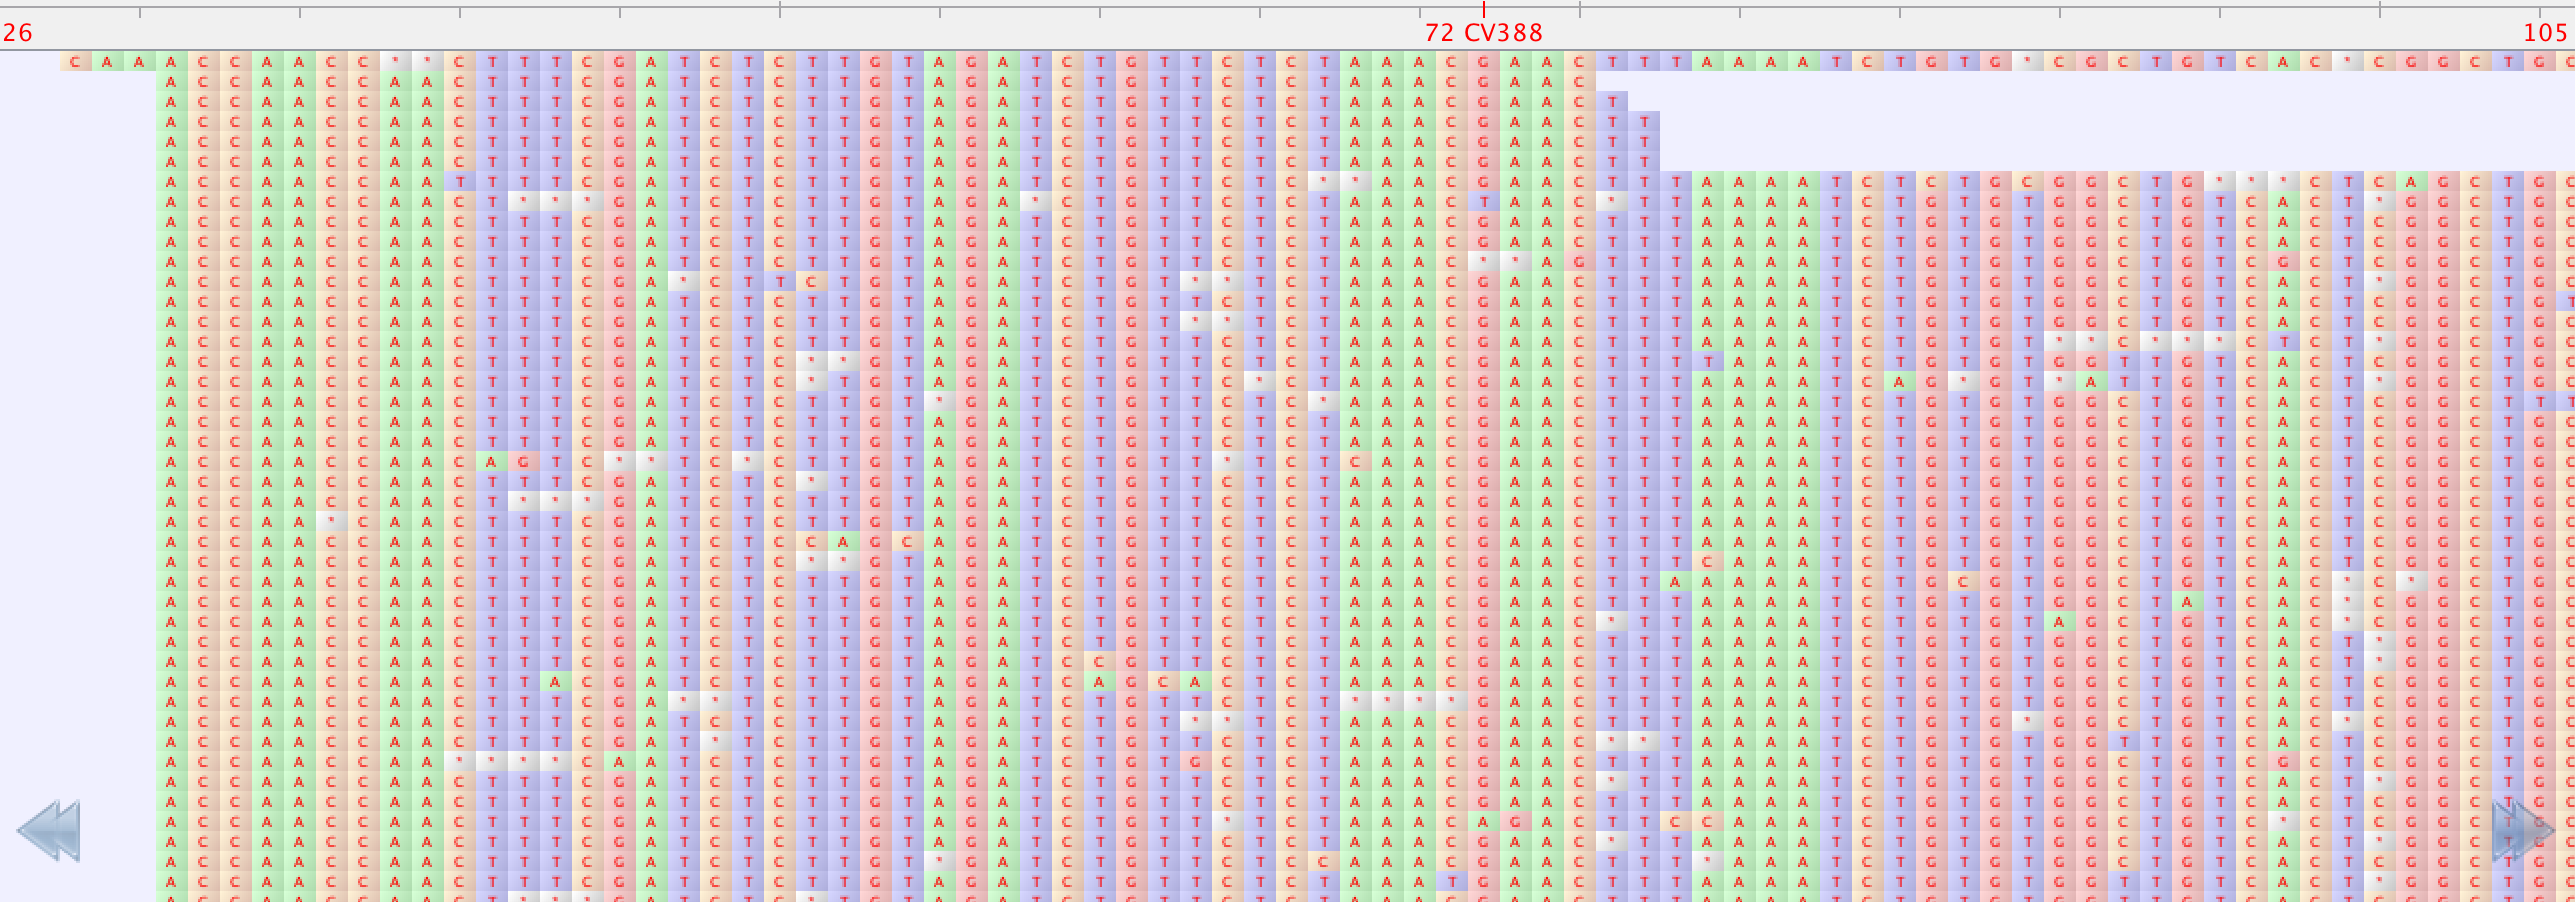
\includegraphics[width=0.99\textwidth]{figs/sam-tablet.png}
\caption{\textbf{SAM file graphical representation.} The software Tablet \comment{ref } was used. The 72th nucleotide in this alignment has a coverage of 388...blabla}
\label{fig:sam}
\end{figure}


\subsubsection{Raw acquisition data}


Although not commonly available, raw acquisition data files can be used to construct probabilistic sequences. Those files usually contain nucleotide signal intensities  as they are read along the DNA/RNA molecular chain. 
For example, Sanger sequencing generates chromatograms (AB1/I files) from variations in fluorescence while nanopores technologies generate electrical resistance signals (FAST5 files). 
Nucleotides are ``called'' from interpreting peaks in the signals. For all technologies, the determination of the nucleotide read from the signal relies on complex and imperfect algorithms (\eg neural networks for nanopore technologies). Rather than a dichotomous translation of the signal into one single nucleotide (potentially associated with an observation error probability using a quality score), it may be beneficial to take a probabilistic approach in calling the bases from raw signal data. 




\newpage

\section{Examples}
\subsection{Propagating sequence uncertainty in phylogeny reconstruction}

Molecular phylogenies are tree-based models that relate common ancestors of genetic sequences. Many sophisticated statistical tools exist to reconstruct phylogenies from genetic material extracted from biological samples. Those statistical methods rely, to a varying degree, on ``truthful'' and accurate observations of molecular sequences, their main -- if not unique -- input data.

Here, we describe our study design to propagate and measure sequence uncertainty in phylogeny reconstruction. 


\subsubsection{Generating simulated probabilistic sequences} 
\label{sec:zanini_poly}

If we want to simulate realistic probabilistic sequence, we have to reproduce a similar uncertainty as the one we would have from either sequencing error or polymorphism. 

We illustrate our methodology in the context of in-host HIV infections. 
The data from Zanini \cite{Zanini:2015} is a good source to assess primarily the diversity of polymorphism for HIV, and to a certain extent too, the sequencing error (because it is always here). 
Briefly, this data set gives, for several patients at several time points during their (untreated) infection, the number of times nucleotides were sample at a given position, across the whole HIV genome. 
The number of nucleotide occurrences at each position can easily be transformed into the probabilities for the probabilistic sequence. The entropy can then be calculated at each position, and also for the entire genome (by simply summing up the entropies for all positions). 

Entropy is a measure of uncertainty. So we can consider the distribution of entropies (for each position on the genome) as a representation of the overall genome sequencing uncertainty, that should be approximately matched by simulations deemed realistic. 
The data from Zanini and colleagues \cite{Zanini:2015} shows that $\nps_{n,j}$, the distribution of base-call probabilities for most positions is highly concentrated just under 1 (which means a high base-call probability for most positions). 
Hence, we choose a Beta distribution to simulate base-call probabilities, and fit the shape parameters $\alpha$ and $\beta$ on the observed entropy distribution:
\begin{equation}
\label{eq:beta_sampling}
S_{n,j} \sim \betadist{\alpha, \beta}
\end{equation}
\begin{equation}
\alpha, \beta \text{ such that } E(\alpha,\beta) = E_{obs}
\end{equation}
where $E$ is the distribution of position-wise entropy.
A fit on Zanini's data \cite{Zanini:2015} gives approximately $\hat{\alpha} = 29.7$ and $\hat{\beta} = 0.06$. \comment{make an appendix to show the details of this fit.}

We calculate the entropy value as 
\begin{equation}
\label{eq:entropyDefinition}
E(\alpha, \beta) = -\sum_{i=1}^{\ell} p_i \log_2(p_i)
\end{equation}
where $p_i$ is the ($\alpha$- and $\beta$-dependent) base-call probability drawn for the nucleotide at position $i$ and $\ell$ is the length of the sequence.




\subsubsection{Assessing the impact of sequencing uncertainty}


Below is our simulation design to study the impact of uncertainty on phylogeny reconstruction.
An illustration of this pipeline is given by \autoref{fig:pipeline}.

\begin{enumerate}
\setcounter{enumi}{-1} 

\item Choose a root sequence of interest (\eg a HIV genome, a random sequence)

\item Generate a phylogeny from this root sequence, using \textsf{phyloSim}. The resulting tree $T^*$ has $n$ tips that represent the sequenced samples $seq_1, seq_2,\ldots, seq_n$. The tree $T^*$ with its sequences $seq_i$ is the ``base'' phylogeny.

\item Add a simulated layer of uncertainty by transforming the ``base'' sequences $seq_i$ into probabilistic sequences $\nps^i$ (for $i=1,2,\ldots,n$).

\item Repeat $M$ times: 
draw a sequence $\widetilde{seq_i}$ for each $\nps^i$ (for $i=1,\ldots, n$).

\item Repeat $M$ times: reconstruct the phylogeny $T_m$ with \textsf{RAxML} from the $(\widetilde{seq_i})_{i=1\ldots n}$. 

\item \label{item:assess} Assess the uncertainty by considering the variance among the phylogenies $(T_m)_{m=1:M}$ using several distance metrics (detailed below).
\end{enumerate}

\noindent Note that the $M$ iterations amounts to a Monte-Carlo algorithm.
Studying the distance between the reconstructed trees $(T_m)_{m=1:M}$ and the true tree $T^*$ is not our main goal (this distance essentially assesses the performance of the phylogeny reconstruction software to correctly infer the ``true'' ancestry).
Instead, we are principally interested in \emph{uncertainty propagation}, that is the variance of the pairwise distances between the $(T_m)_{m=1:M}$.

Our analysis considers five levels of uncertainty. We start with a virtually inexistent sequence uncertainty, then increased it by lowering the base call probability. This is done by sampling the probability from multiple parameter sets $(\alpha,\beta)$ of a Beta distribution (see \autoref{eq:beta_sampling}). 
We choose a single value $\alpha=29$ and use five different values for the second shape parameter $\beta = 10^{-3}, 10^{-2}, 10^{-1}, 1 \text{ and } 3$ \comment{update if necessary}.
With these values, the mean of the Beta distribution for the base-call probability decreases away from 1.0. 
Finally, note that the middle value $(\alpha=29, \beta=10^{-1})$ is close to the fitted entropy values of the longitudinal HIV dataset from Zanini and colleagues \cite{Zanini:2015}.

For Step \ref{item:assess}, we explore the impact of sequence uncertainty on several types of downstream analysis on reconstructed phylogenies: pairwise distance between trees, clustering and an example of source attribution \comment{amend if needed}.


\textbf{Pairwise distances between trees.}
Define the set 
\begin{equation}
D = \{d(T_i,T_j);\,\, i=1,\ldots, M \text{ and } j<i \}
\end{equation}
with $d$ a tree distance. 
%$D$ has ${M(M-1)/2}$ data points. 
The distance $d$ should be a statistically-convenient metric that represents faithfully the differences of interpretation (\ie uncertainty) of phylogeny reconstruction. 
We use three distances:  Robinson-Foulds (RF) \cite{Robinson:1981}, kernel \cite{Poon:2013} and a label-based distance \cite{xxx}. 
% We expect the mean (and variance) of $D$ to increase as the sequencing uncertainty increases. 

We measure the uncertainty of phylogenetic inference with the coefficient of variation $c = s / m$ where $m$ is the mean of $D$ and $s$ its standard deviation.
We note $c_{RF}$, $c_K$ and $c_{L}$ the coefficients of variation calculated with the RF, kernel and label-based distances, respectively.

Although not our primary objective in this study, we also investigate the distance of the inferred tree $T_i$ to the benchmark tree $T^*$, and define 
\begin{equation}
D^* = \{d(T_i,T^*);\,\, i=1,\ldots, M \} 
\end{equation}
Similarly as for $c$, we define $c^*$ as the coefficient of variation of $D^*$ and adopt the same subscript notation to differentiate between the distances used for its calculation.



\begin{figure}[ht]
\centering
    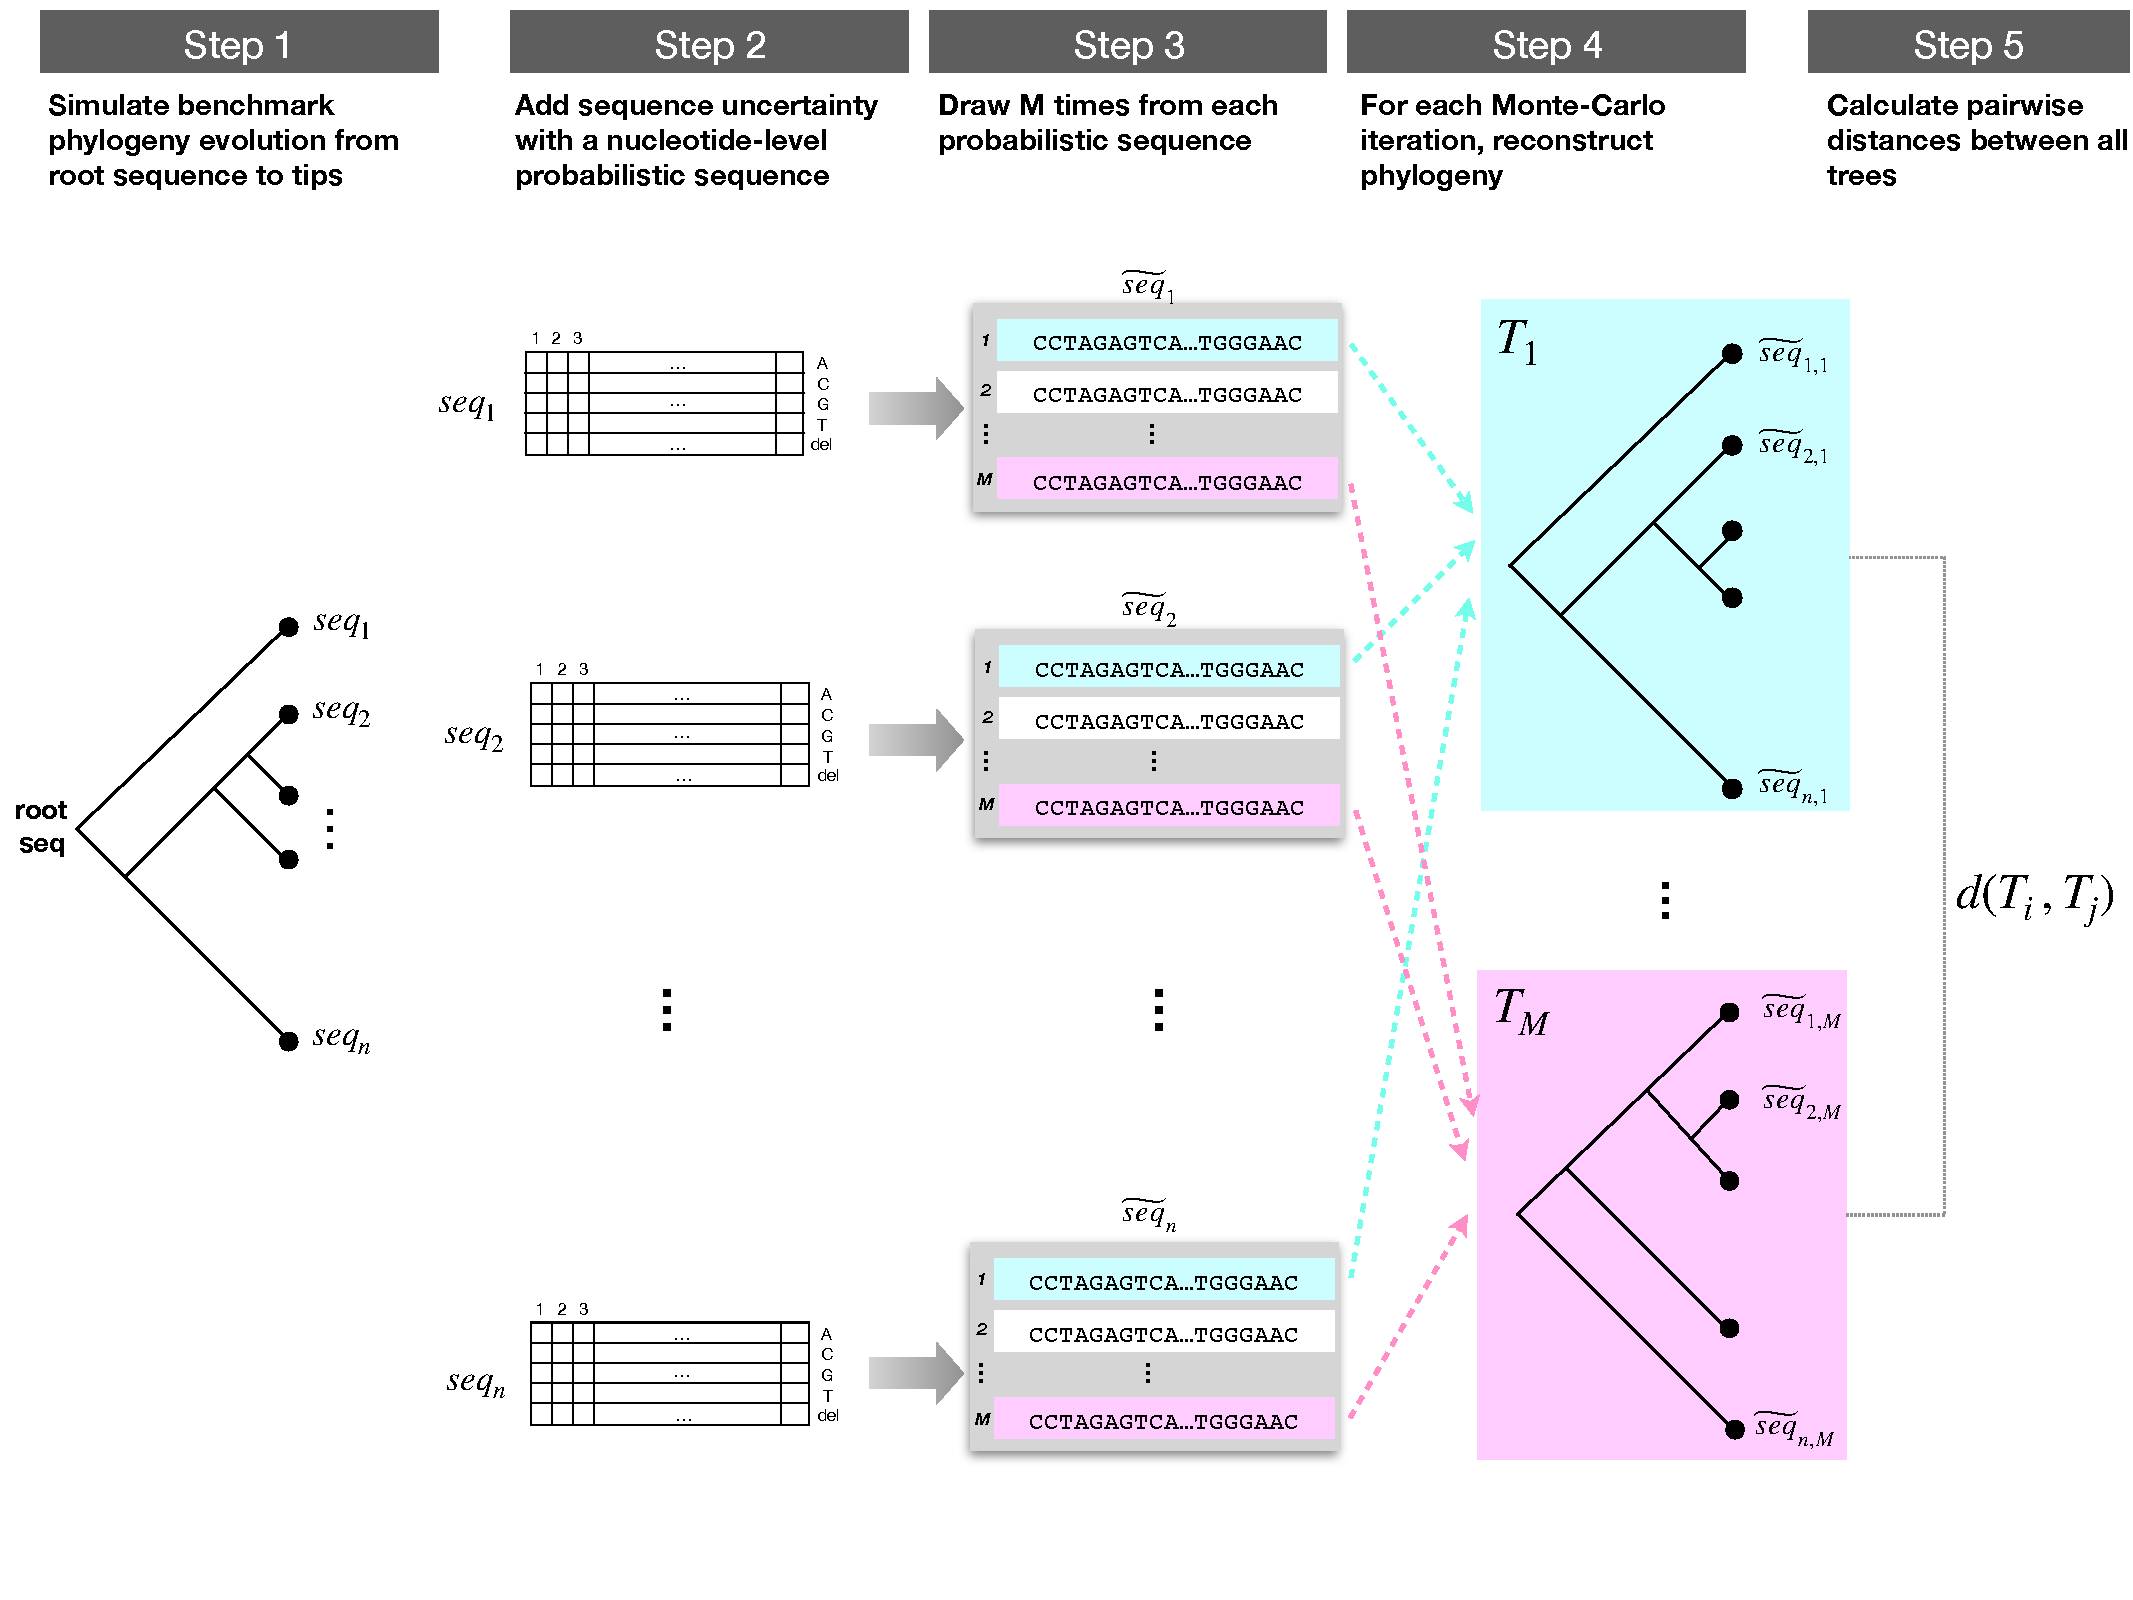
\includegraphics[width=0.99\textwidth]{figs/pipeline.pdf}
\caption{\textbf{Simulations pipeline.} 
\textit{Step 1}: A phylogeny with $n$ final nodes is simulated from a root sequence using \textsf{phylosim}.
\textit{Step 2}: A \nlps is generated for each sequence, assuming a Beta distribution for the base-call probability
\textit{Step 3}: For each \nlps, a sequence is drawn $M$ times
\textit{Step 4}: Using the ith drawn sequence (\ie ith Monte Carlo iteration), the phylogeny $T_i$ is inferred ($i=1,\ldots,M$). 
\textit{Step 5}: The pairwise distances $d(T_i, t_j)$ are calculated for all $i<j$.
Steps 1 to 5 are repeated for several level of uncertainty (defined by the Beta parameters of the base-call probabilities).
}
\label{fig:pipeline}
\end{figure}


\textbf{Impact on clustering.}
\warning{TODO}

\textbf{Impact on source attribution.}
\warning{TODO}

%Labeled distance: Tree distances are relatively ``generic''. 
%Given our phylogenic framework, more ``practical'' measure could be useful (?). 
%For example, for a given terminal node (tip, leaf) A, how does the probability that it shares a direct common ancestor with B evolve as we increase uncertainty?





\newpage
\section{Results}

\newpage
\bibliography{papers}
\end{document}  